\documentclass[12pt]{article}
\usepackage{graphicx}
\usepackage{float}
\usepackage{geometry}
\usepackage{fontspec}
\usepackage{hyperref}

\hypersetup{
colorlinks=true,
linkcolor=blue,
filecolor=blue,      
urlcolor=blue,
citecolor=cyan,
}

\geometry{a4paper, left=2.54cm, right=2.54cm, top=2.54cm, bottom=2.54cm}
\setmainfont{Times New Roman}
\linespread{1.5}

% COVER

\begin{document}
\begin{titlepage}
    \centering
    
\includegraphics[width=0.6\textwidth]{Logo.png}\par\vspace{1cm}
    \vspace{1cm}
    {\scshape\LARGE Research on Fall Detection System for the Elderly and Its Potential\par}
    \vspace{2.5cm}
    {\Large Coursework 3: Literature Review\par}
    \vspace{6cm}
    {\Large Wenxuan Zhu(20379163)\par}
    \vspace{0.5cm}
    {\Large alywz30@nottingham.ac.uk\par}
    \vfill
    {\Large April 2023\par}
\end{titlepage}

% MAIN BODY
\section{Introduction and Motivation}

With the serious problem of population aging, more and more elderly people living alone have or will appear in the future. For their children, their real-time safety issues are a very important aspect to consider. After the elderly lose their mobility, it is difficult to contact the outside world for help in a timely manner. Even if the surveillance cameras can observe in real time, their children cannot continue to observe. Especially at night, the monitoring cameras basically lose their function, if the elderly drop down from the bed, it will be a big security risk.
\\ \hspace*{\fill} \\
Based on this, thermal camera can be an effective way to be used in this situation. A Thermal camera can clearly photograph and display people's behaviour at night. Hence, by using the thermal camera, we can design a project which aims to design a system to monitor the position and posture of an elderly who is lying on the bed alone and alert the injury of their dropping down from the bed at night. 
\\ \hspace*{\fill} \\
After planning the content of the project, we first need to study some existing literature, which may be completely similar or related in a certain field, which can not only prevent us from duplicating research, but also give us research direction and the method brings some guidance and help, so as to broaden our horizons and see more application aspects and possibilities. Therefore, the Fall Detection System for the Elderly seems to be a more accurate entry point for the research and evaluation of this project. It is not limited to thermal imaging recognition, and there is no specified time, which can bring greater retrieval space and possibilities. gender assessment. I found 10 papers related to this topic, and the distribution of their publication years and numbers is shown in Figure 1:

\begin{figure}[H]
\centering
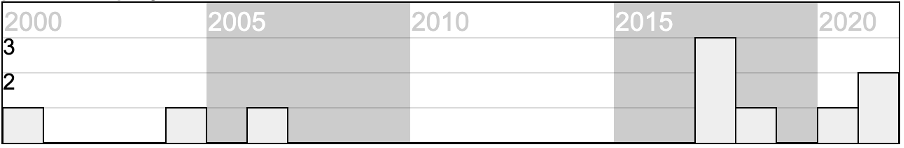
\includegraphics[width=0.7\textwidth]{meta-data.png}
\caption{Number of papers by publication year} 
\end{figure}

\noindent In order to more clearly show the types and areas of focus of these documents, Figure 2 shows more features of the documents more intuitively:

\begin{figure}[H]
\centering
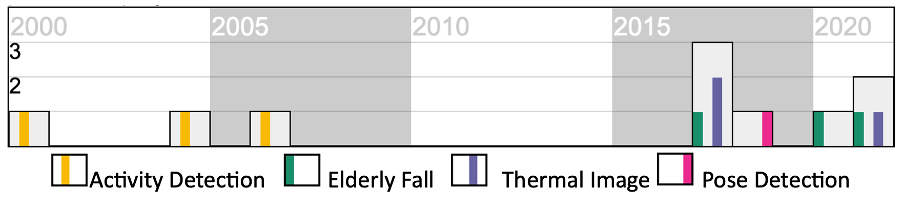
\includegraphics[width=0.7\textwidth]{supplementary-figure.png}
\caption{Number of papers by publication year and focus areas} 
\end{figure}

\noindent There are 10 papers in total. We stopped searching for literature in the middle of 2021.

\subsection{Field Challenges}

There are many common challenges in the topic of Fall Detection System for the Elderly. The first challenge is the recognition of fall detection. At present, there are many solutions for detection and recognition. The mainstream methods focus on sensor detection and image detection(Wang, 2020). But it is still impossible to find the solution with the highest accuracy rate because the focus of the two detections is different. The former pays more attention to the logical judgment of multiple sensors, while the latter pays more attention to the algorithm(Cheung, 2021). In addition, different acquisition tools will affect the results, so this is the biggest challenge at present.
\\ \hspace*{\fill} \\
Secondly, time is also a relatively big challenge. There is no specific period that will cause relatively large challenges to the system. For example, in image detection, the night environment will affect the camera, so it is necessary to select a specific night imager to solve it. In addition, run time also has an impact on the life and sensitivity of the sensor.
\\ \hspace*{\fill} \\
Finally, there is the problem of crowd recognition. How to judge that the person detected by the system is an elderly person is a relatively big challenge.

\subsection{Survey Scope}

This article will summarize, analyze and summarize the 10 collected documents. These include the identification method and implementation steps of the elderly's fall, the analysis method and algorithm of ordinary imaging and thermal imaging photos in image recognition, and the identification and analysis of some special posture behaviors. It is worth adding that this paper does not include the definition and identification of target populations, nor does it include exploring the impact of the temporal dimension.

\subsection{Search Methodology}

There are two main ways to collect 10 relevant research documents in this paper. The first is to search for similar articles or highly relevant articles in the academic library according to keywords, and the second is to search and expand in ConnectedPapers.com Related research literature, as shown in Figure 3:

\begin{figure}[H]
\centering
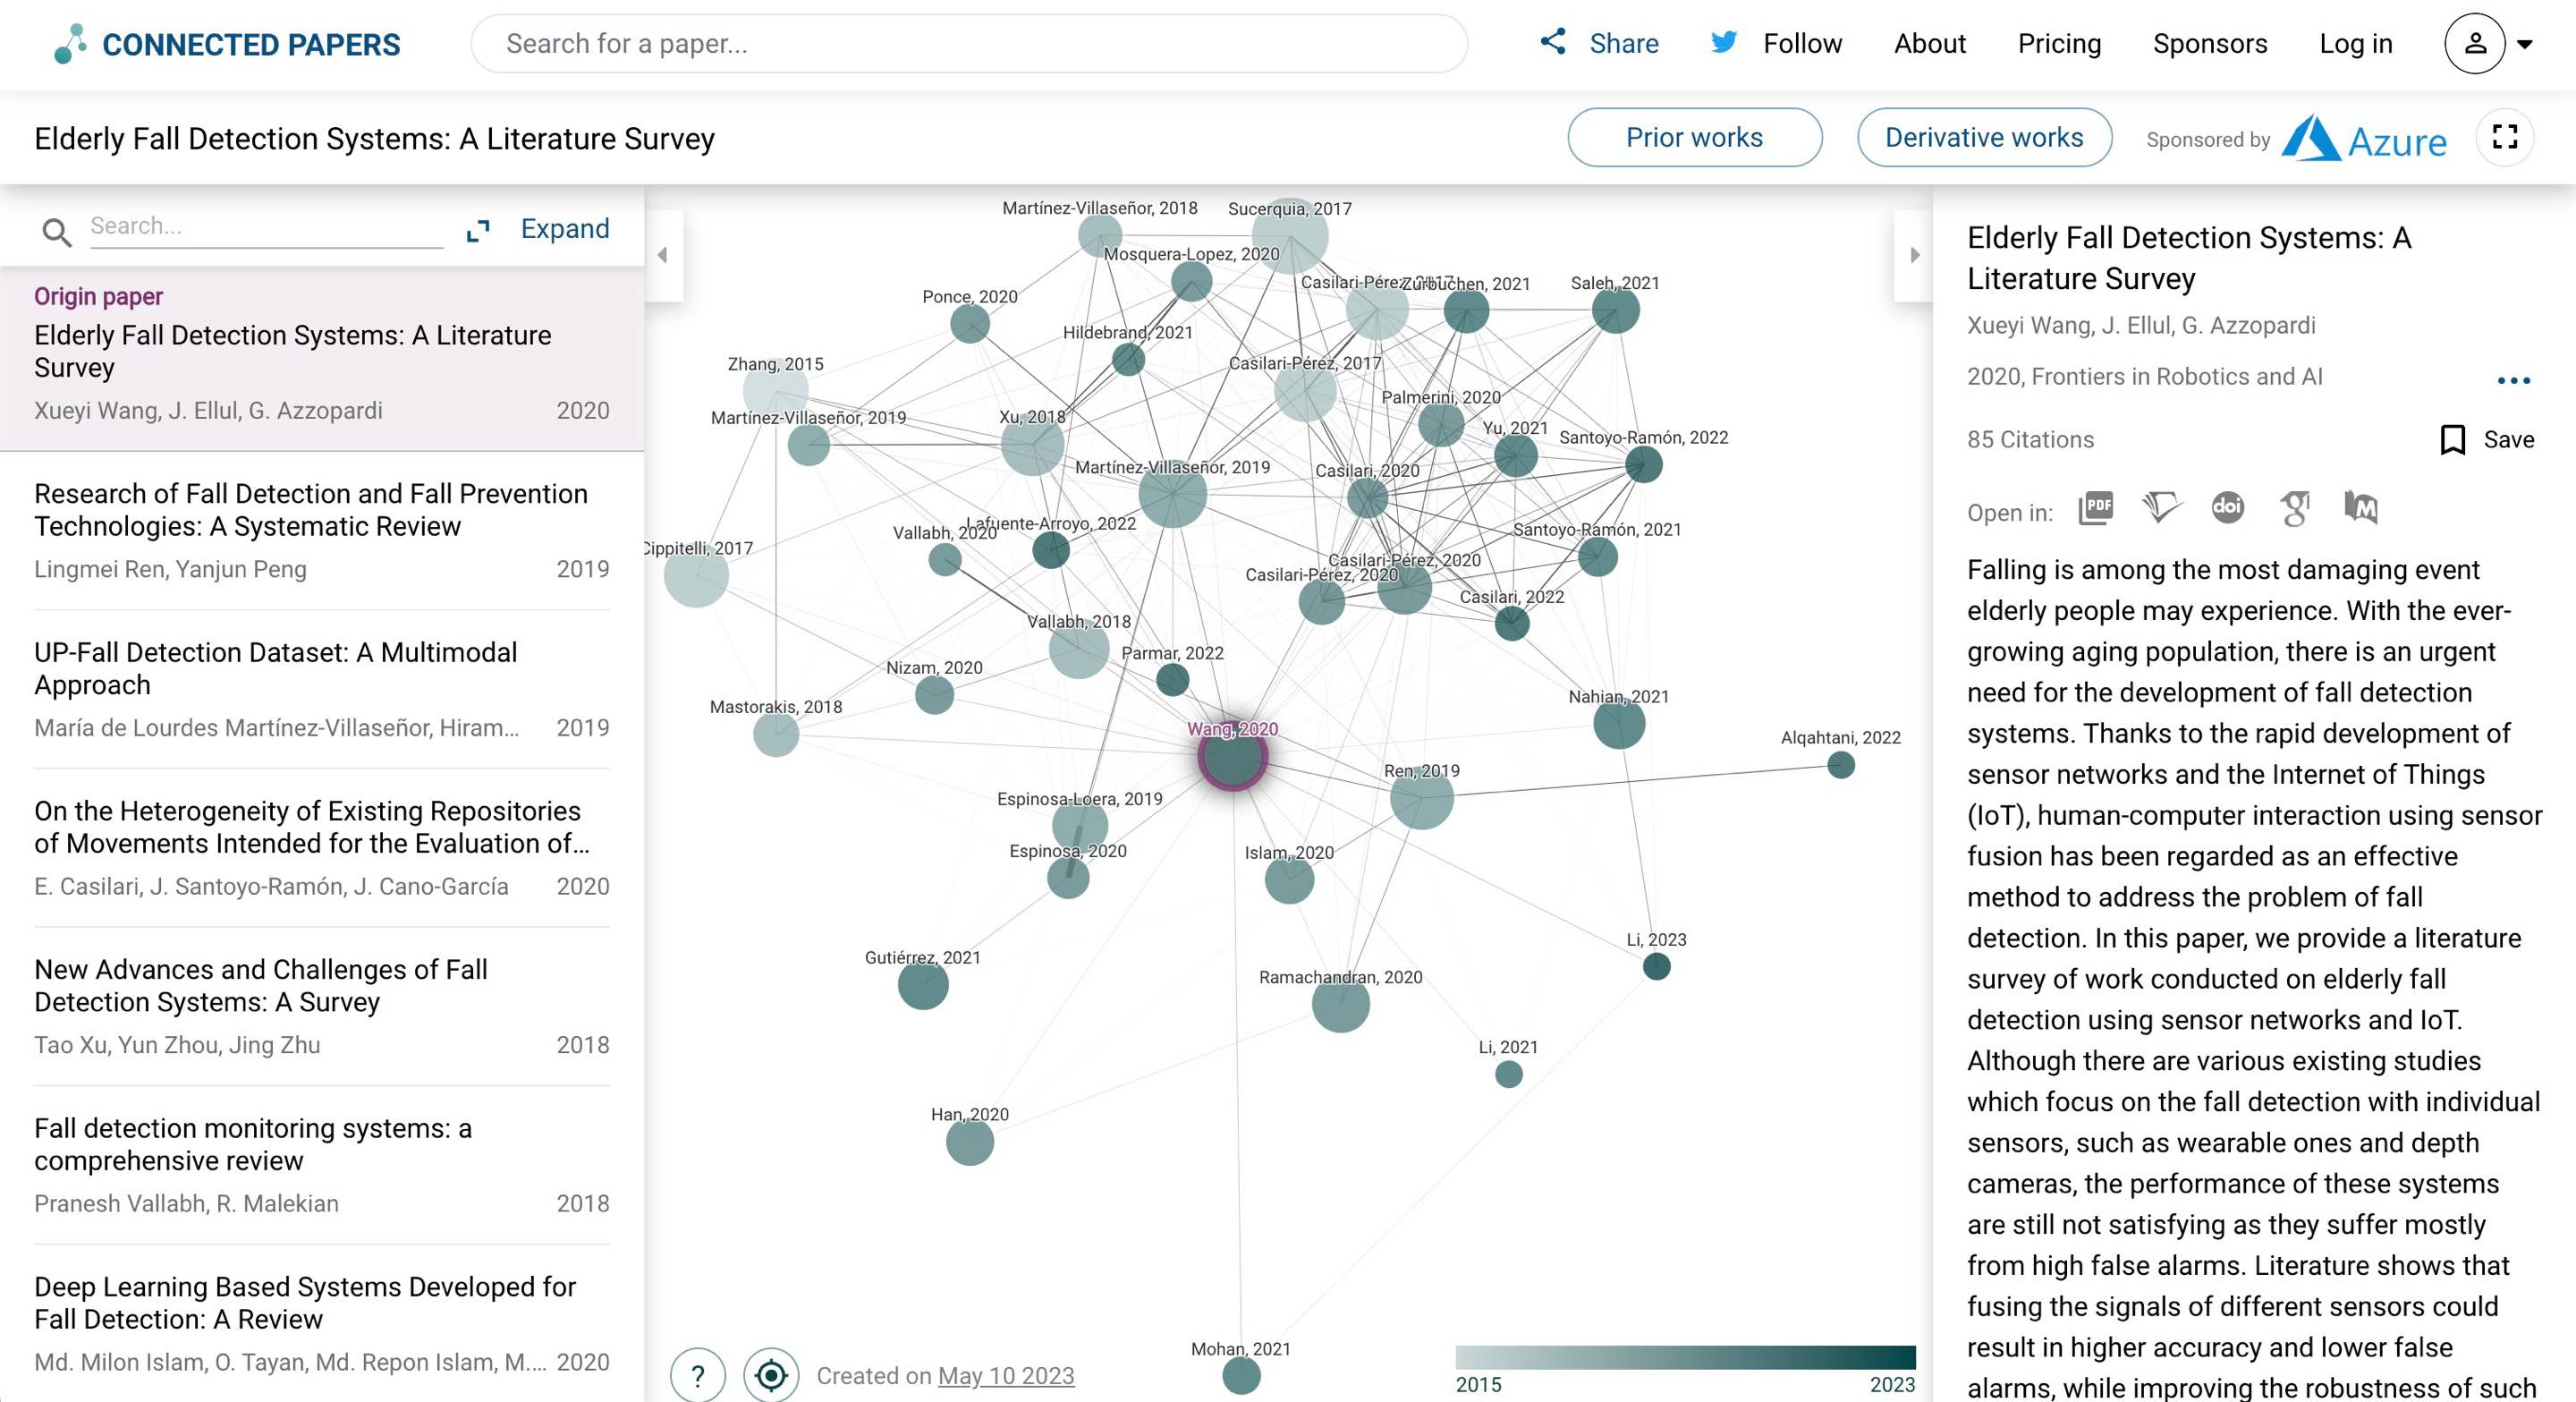
\includegraphics[width=1\textwidth]{connected-paper.pic.jpg}
\caption{ConnectedPapers.com} 
\end{figure}

\subsection{Classification of Literature and Organization}

The 10 papers can be divided into 4 categories according to their focus areas and research directions, including activity detection, elderly fall, thermal image and pose detection.Figure 2 clearly shows the categories and dimensions of these documents.

\begin{figure}[H]
\centering
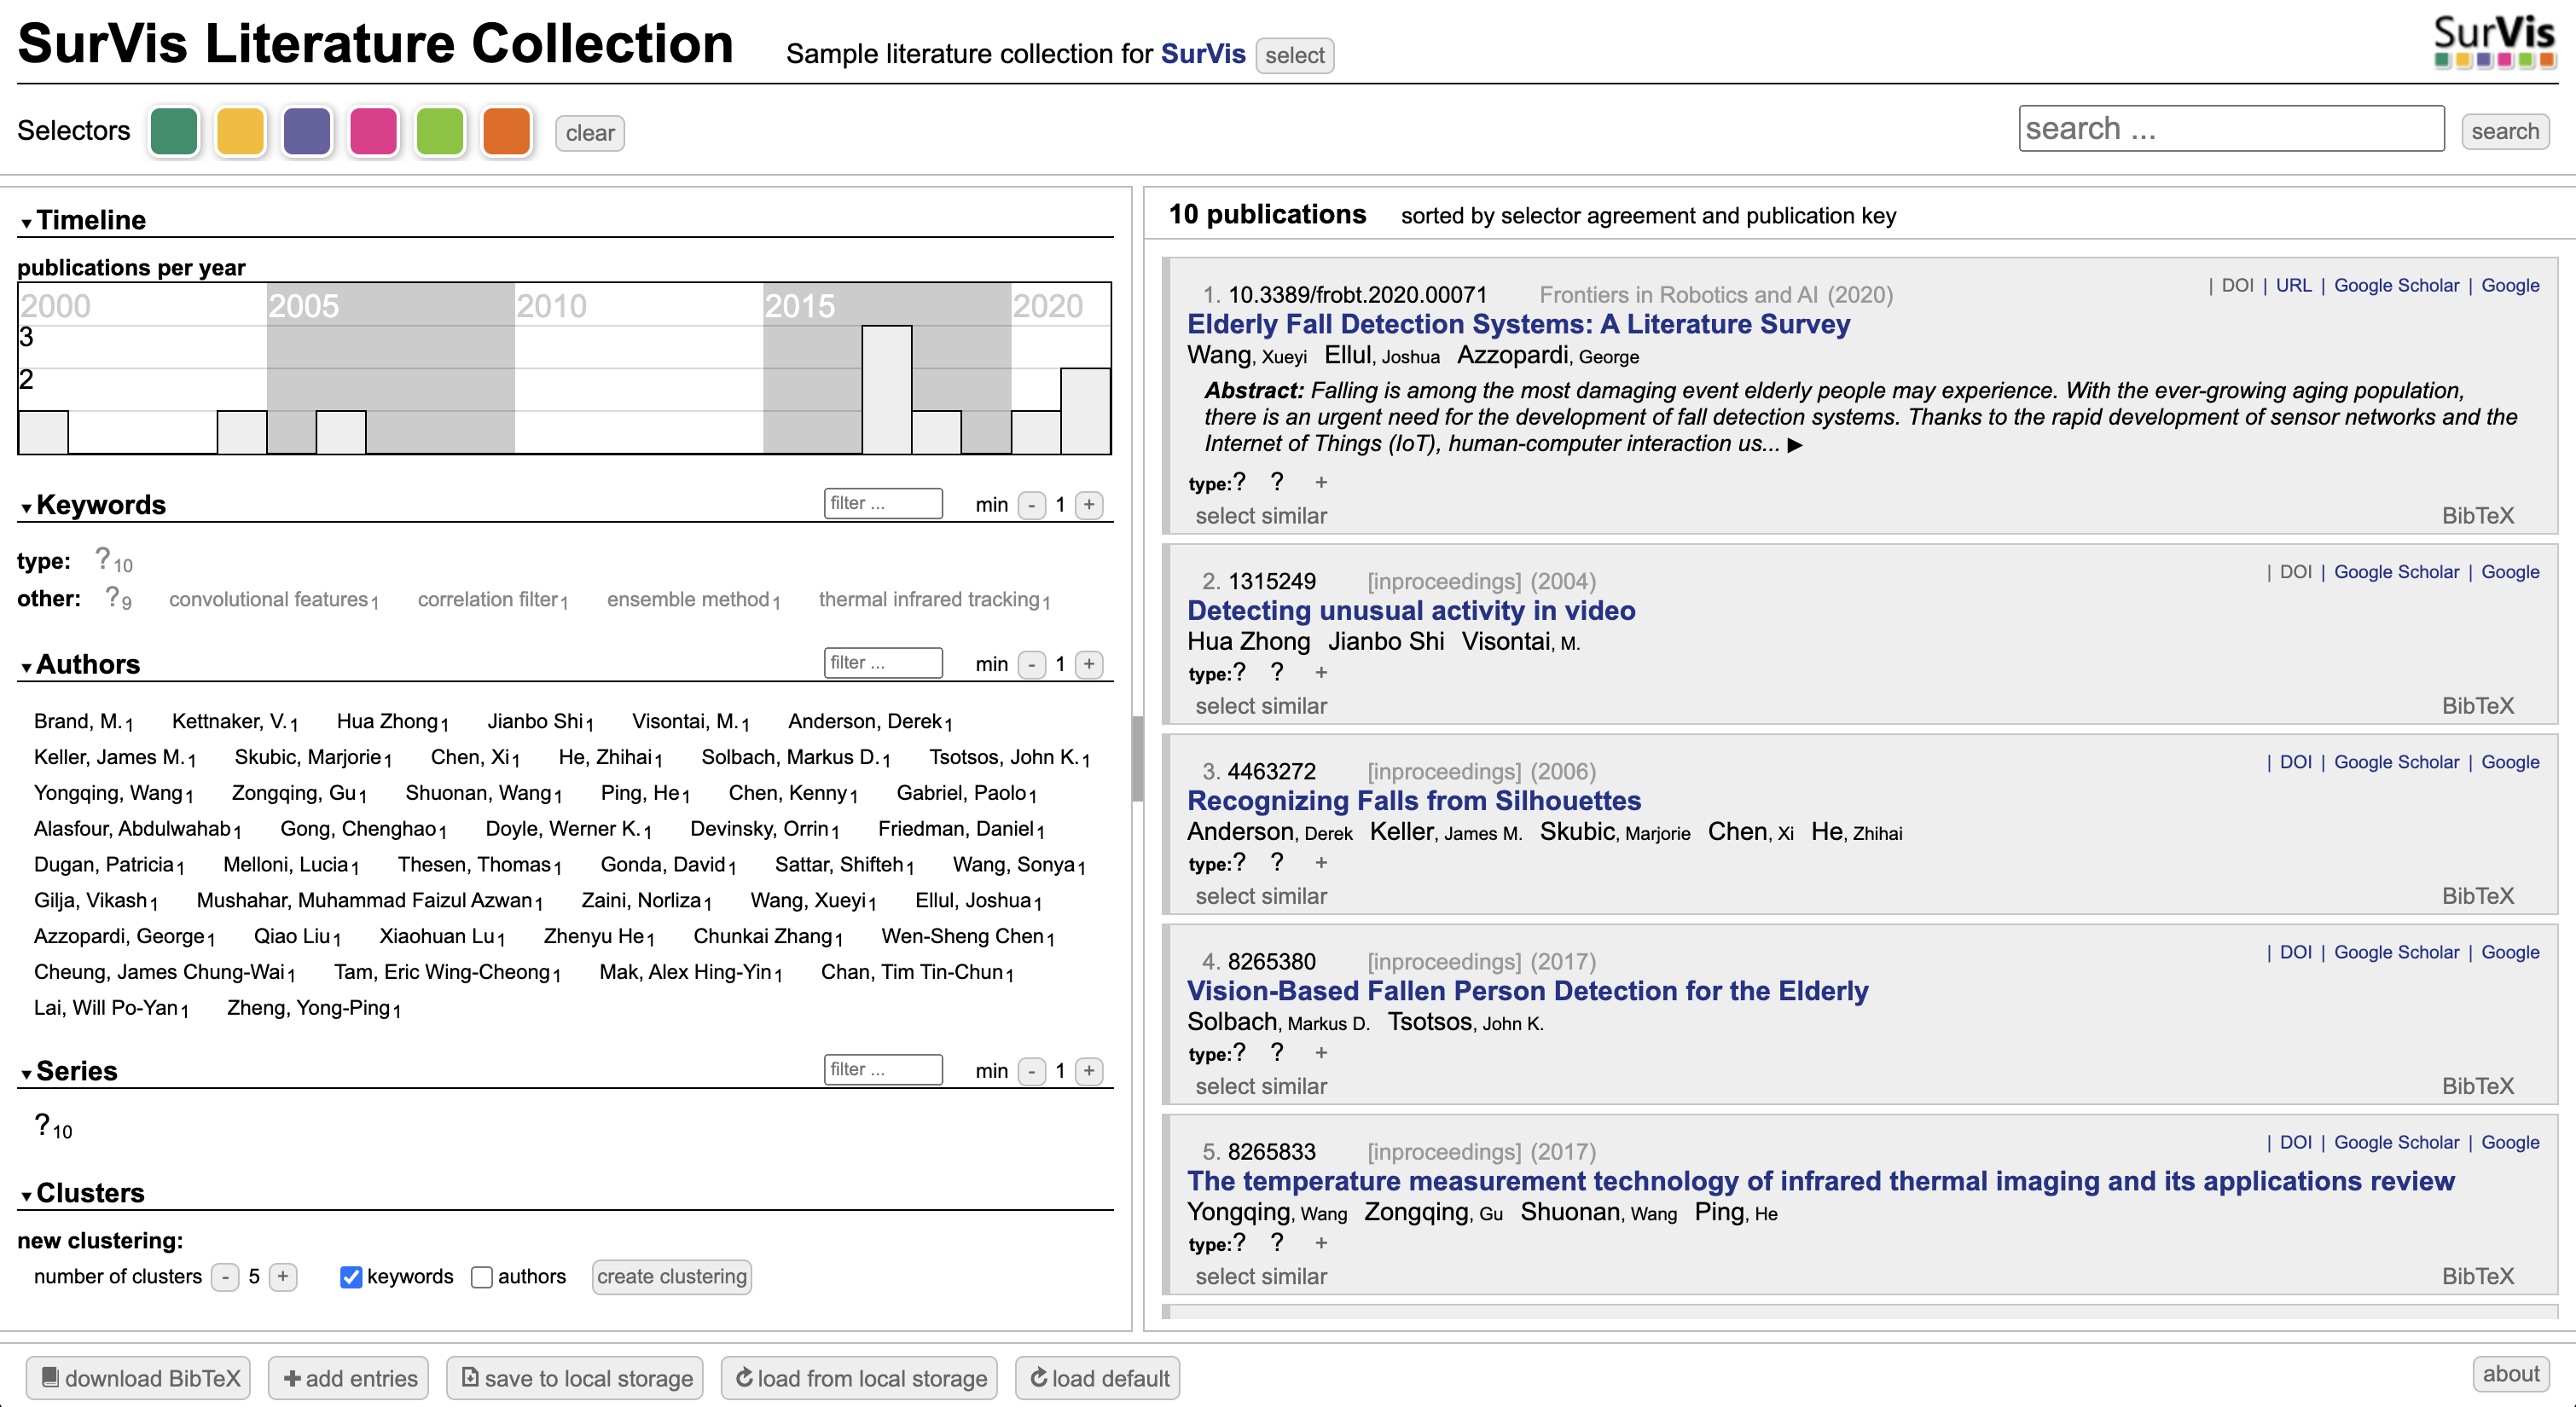
\includegraphics[width=1\textwidth]{survis.pic.jpg}
\caption{SurVis literature collection} 
\end{figure}

\noindent As shown in Figure 4, this is my Survis literature browser web page and the URL of it is as follow:
\url{https://hennnnnry.github.io/survis/survis_0.1.0_20151022/src/index.html}

\section{Paper Summaries}

This paper collects 10 literatures that are highly relevant to the fall detection system for the elderly. The summary of each literature is as follows:
\\ \hspace*{\fill} \\
\textbf{Elderly Fall Detection Systems: A Literature Survey}

\noindent This article collects, investigates, evaluates and summarizes the fall detection of the elderly based on sensor and Internet of Things technology, including related work and research, and points out the direction of future efforts and possible beneficial areas(Wang, 2020). The Implementation of this document is mainly achieved by analyzing and summarizing the technical level of existing documents, the process from data collection to analysis and security. The surge in the aging population has led to an increasing demand for fall detection and prediction in the elderly(Bloom, 2011), which is the core related work of this literature. It uses 2D data, distributed in time and space, and presented numerically. Furthermore, it is evaluated through literature survey and data comparison.Its representative image is as follows:

\begin{figure}[H]
\centering
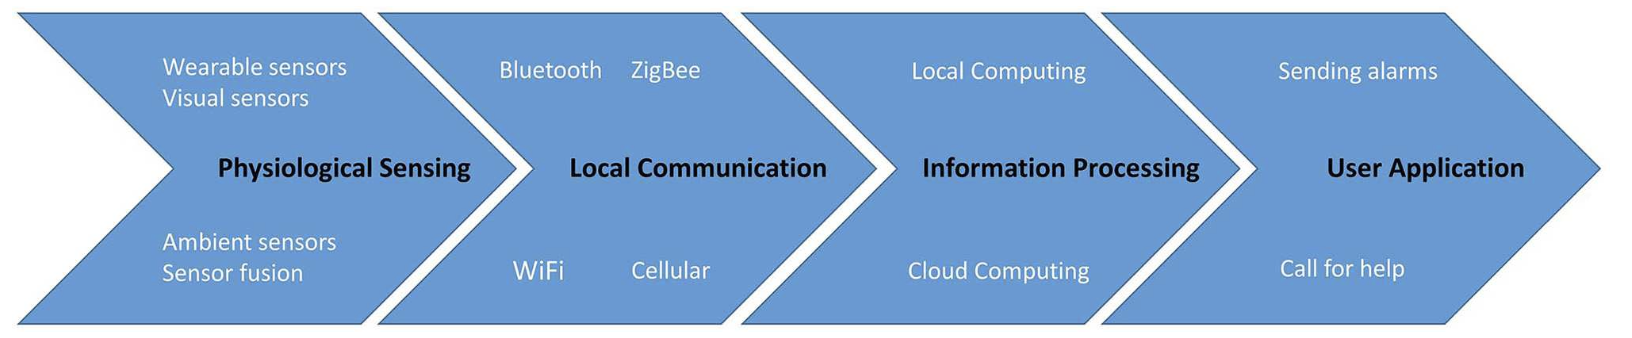
\includegraphics[width=1\textwidth]{Paper1.pic.jpg}
\caption{Main components of a fall detection system} 
\end{figure}

\noindent \textbf{Recognizing Falls from Silhouettes}

\noindent This paper mainly starts from the computer image point of view, based on color segmentation for silhouette recognition and shadow removal, to recognize the fall detection of the elderly(Anderson, 2006). The implementation of this document is mainly carried out by proposing back segmentation and recognition, extracting silhouettes, training hidden Markov models, testing and obtaining experimental data and result analysis and discussion. By using an unsupervised method, imitating document keyword analysis, combining many simple features, and using this to analyze and judge an activity(Zhong, 2004), this is the core related work of this document. It includes image presentation and 2D data analysis in computer vision, as well as some vector graphics. Furthermore, it is evaluated through simulation and real experimental cases. Its representative image is as follows:

\begin{figure}[H]
\centering
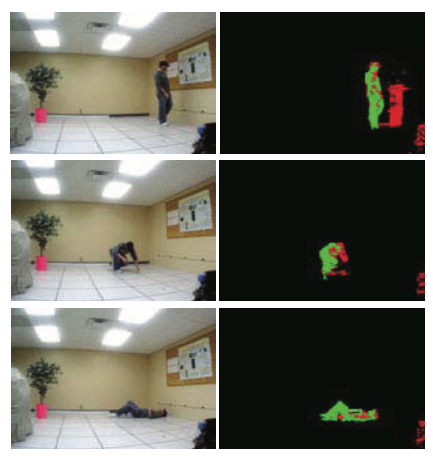
\includegraphics[width=0.7\textwidth]{Paper2.pic.jpg}
\caption{Silhouette extraction results} 
\end{figure}

\noindent \textbf{Night-Time Monitoring System (eNightLog) for Elderly Wandering Behavior}

\noindent This document proposes the development of a nighttime monitoring system called eNightLog, which aims to solve the common behavior disorder of the elderly in the community called wandering and can reduce the workload of caregivers and reduce the psychological impact of physical solutions on the elderly(Cheung, 2021). The implementation of this document is mainly carried out through the steps of sensor selection, system construction, experimental verification, and algorithm accuracy analysis. The behavioral disturbance of the elderly at night will have negative impacts on themselves and the caregivers, and the false positives and limitations of the sensor also need to be improved(Ranasinghe, 2014), which is the core related work of this literature. It contains some 3D data and numerical formulas, including the division of hierarchical dimensions. Furthermore, it is evaluated through experimental validation cases and algorithm comparisons. Its representative image is as follows:

\begin{figure}[H]
\centering
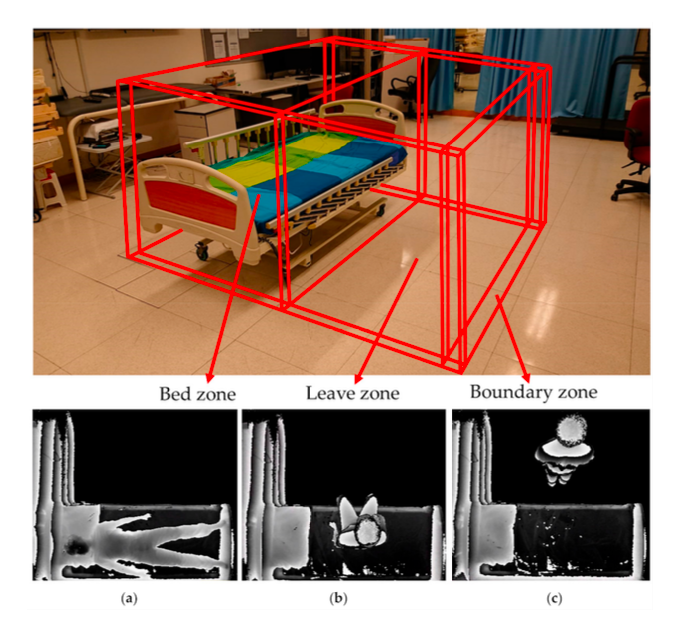
\includegraphics[width=0.7\textwidth]{Paper3.pic.jpg}
\caption{eNightLog system captures images} 
\end{figure}

\noindent \textbf{Vision-Based Fallen Person Detection for the Elderly}

\noindent This paper proposes a CNN-based human fall detector that combines stereo data with a neural network-based human pose estimator for inference(Markus, 2017). The Implementation of this document is mainly carried out through the steps of related technical background analysis, algorithm system construction, logic flow introduction and experimental calculation verification. By using human posture to judge whether the old man has fallen, the human posture estimator has given very strong theoretical support(Noury, 2007), which is the core related work of this document. It contains 3D spatial data, as well as 2D chart data, including vector data and numerical data, which increases the spatial dimension. Furthermore, it is evaluated by studying algorithm documentation sets and experimental case validation. Its representative image is as follows:

\begin{figure}[H]
\centering
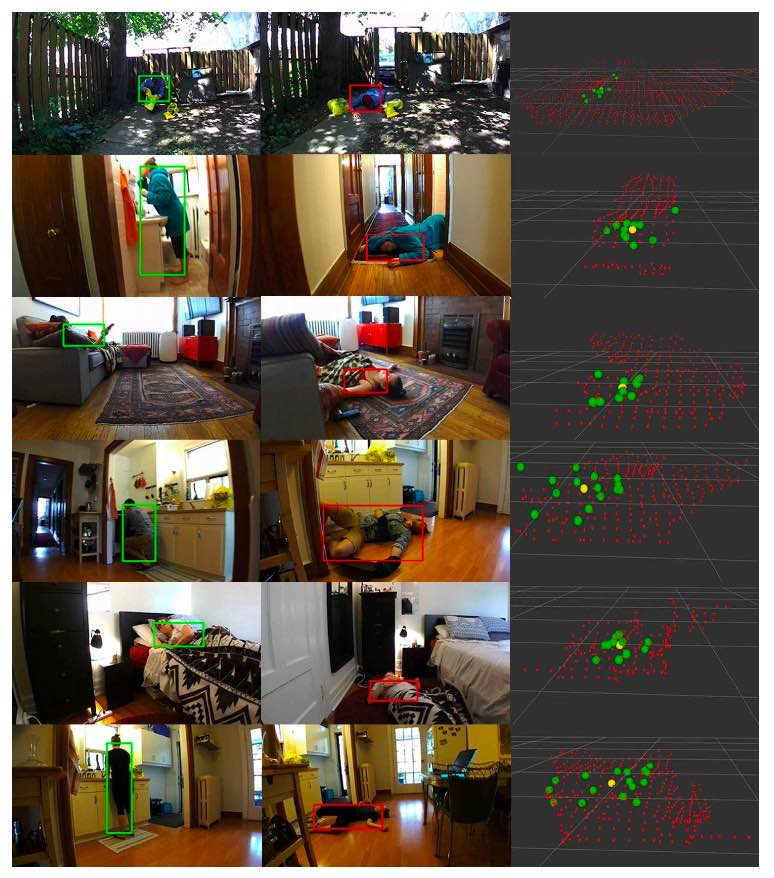
\includegraphics[width=0.7\textwidth]{Paper4.pic.jpg}
\caption{Experimental photos in a home environment} 
\end{figure}

\noindent \textbf{Discovery and Segmentation of Activities in Video}

\noindent This paper proposes that in order to detect anomalous behavior and infer hidden states in low-bitrate encoded activity scenes, the internal state machine of the HMM can be exploited to convert observed activities into meaningful states by minimizing the entropy of the joint distribution(Brand \& Kettnaker, 2000). The Implementation of this document is mainly carried out through the steps of algorithm introduction, example verification and experimental training verification. The application of HMMs and HMM-based hybrids in the field of computer vision is very mature. It mainly focuses on spoken language and gesture recognition, but its cost performance is relatively low(Jelinek, 1998). This is the core related work of this document. It contains a lot of 2D and 3D data, most of which are presented in the form of numerical values and space vectors, and spatial dimensions and pixel calculations are also included. Furthermore, it evaluates by studying algorithm documentation, comparison with similar algorithms, context-specific case studies, and experimental case validation. Its representative image is as follows:

\begin{figure}[H]
\centering
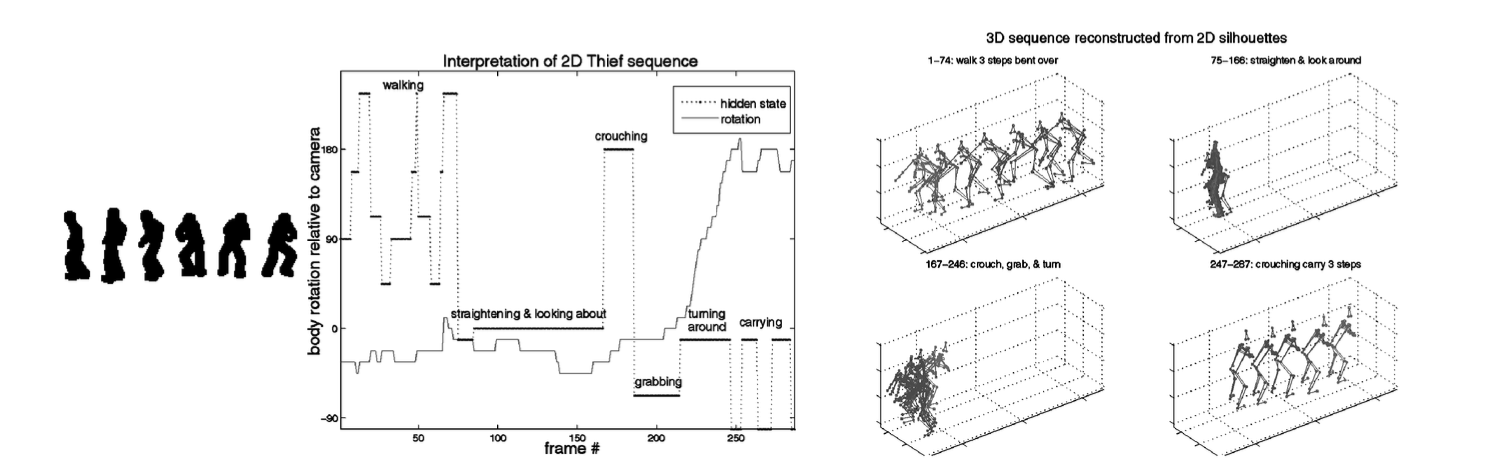
\includegraphics[width=0.7\textwidth]{Paper5.pic.jpg}
\caption{Silhouette infers hidden state sequences} 
\end{figure}

\noindent \textbf{Detecting Unusual Activity in Video}

\noindent This paper proposes an unsupervised technique that divides videos into equal-length segments, performs feature classification, and calculates the prototype-segment co-occurrence matrix to detect abnormal activities in videos(Hua, 2021). The Implementation of this document is mainly carried out through the steps of model introduction, feature selection, algorithm introduction analysis and experimental reproduction verification. Generally speaking, the detection of abnormal events is achieved through video extraction and tracking of object movement and description of abnormal activity characteristics(Wren, 1997), which is the core related work of this document. It mainly contains some 2D and 3D data, which are displayed in the form of vectors and pixels, supplementing the information of the time dimension, and some experimental data are time sensitive. Additionally, it is evaluated by studying algorithm documentation, mathematical proofs, and experimental case verification. Its representative image is as follows:

\begin{figure}[H]
\centering
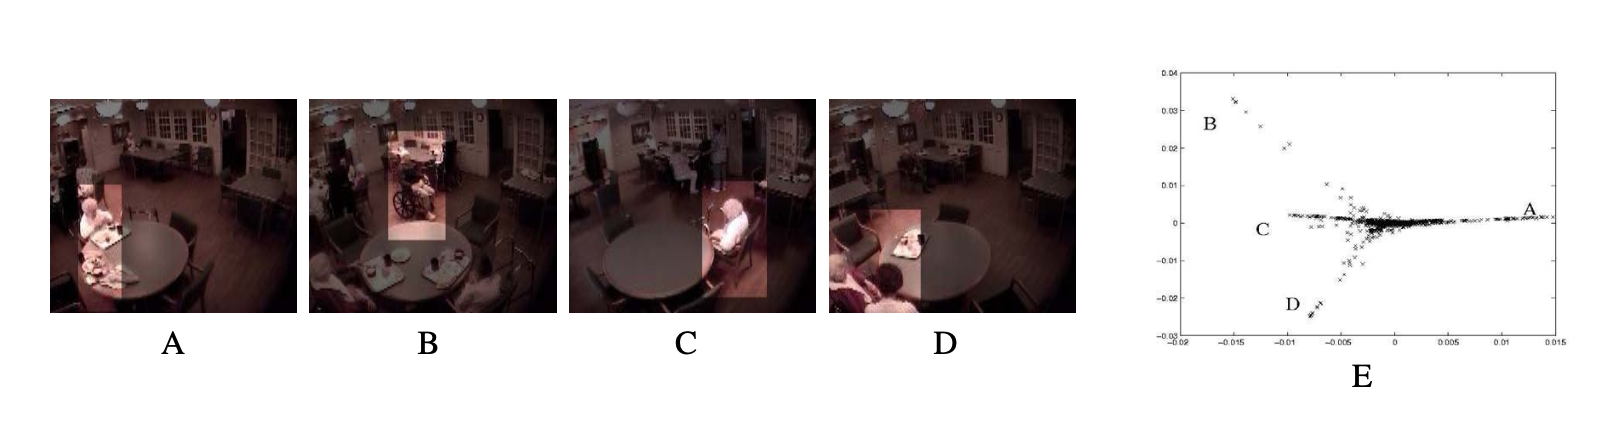
\includegraphics[width=0.7\textwidth]{Paper6.pic.jpg}
\caption{Long-range clusters in the embedded space corresponding to four unusual activities} 
\end{figure}

\noindent \textbf{Human Body Temperature Detection based on Thermal Imaging and Screening using YOLO Person Detection}

\noindent This document proposes a human body temperature detection system based on the You Only Look Once (YOLO) model and the OpenCV library, which combines the temperature detection of thermal imaging with the object detection method of image processing, which greatly improves the detection accuracy(Mushahar \& Zaini,2021). The implementation of this document is mainly carried out through the background introduction of the advantages and disadvantages of thermal imaging, the explanation of the system process steps and the experimental test results. Thermal imagers can not only screen test objects in a short period of time but can also operate remotely to measure the temperature in a large area, but they cannot effectively avoid the interference of other factors such as objects(Hageman, 2019). This is the core related of this document work. It contains 2D data, mainly focusing on the display of temperature and color, and increases the spatial dimension to facilitate the capture of space vectors. Furthermore, it is evaluated through performance comparisons with single algorithms, case studies for specific scenarios, and experimental case validation. Its representative image is as follows:

\begin{figure}[H]
\centering
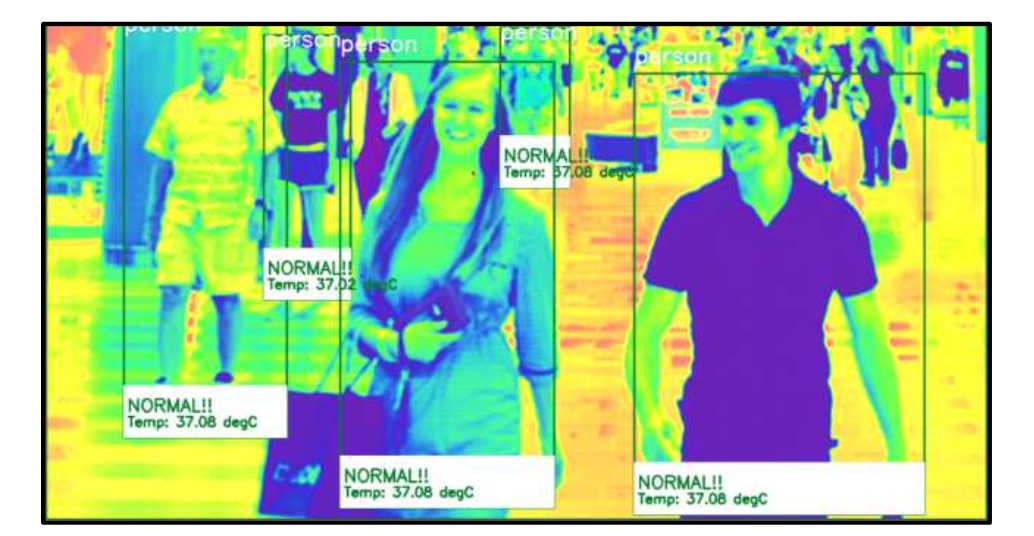
\includegraphics[width=0.7\textwidth]{Paper7.pic.jpg}
\caption{Temperature measurement in premises} 
\end{figure}

\noindent \textbf{The temperature measurement technology of infrared thermal imaging and its applications review}

\noindent This document aims to introduce the principle and parameters of infrared thermal thermometry technology, summarize the application research, and look forward to the future development direction(Wang, 2017). The Implementation of this document is mainly carried out by summarizing the applications of infrared thermal imaging in fields such as medical treatment, energy, and construction. Infrared thermal imagers generally consist of three parts: an infrared detector, an optical imaging system, and an optical scanning system. There is a fixed calculation formula for the corresponding temperature(Li, 2010). This is the core related work of this document. It does not contain multidimensional data but has some mathematical formulas. Furthermore, it is evaluated through case studies of different domain-specific scenarios. Its representative image is as follows:

\begin{figure}[H]
\centering
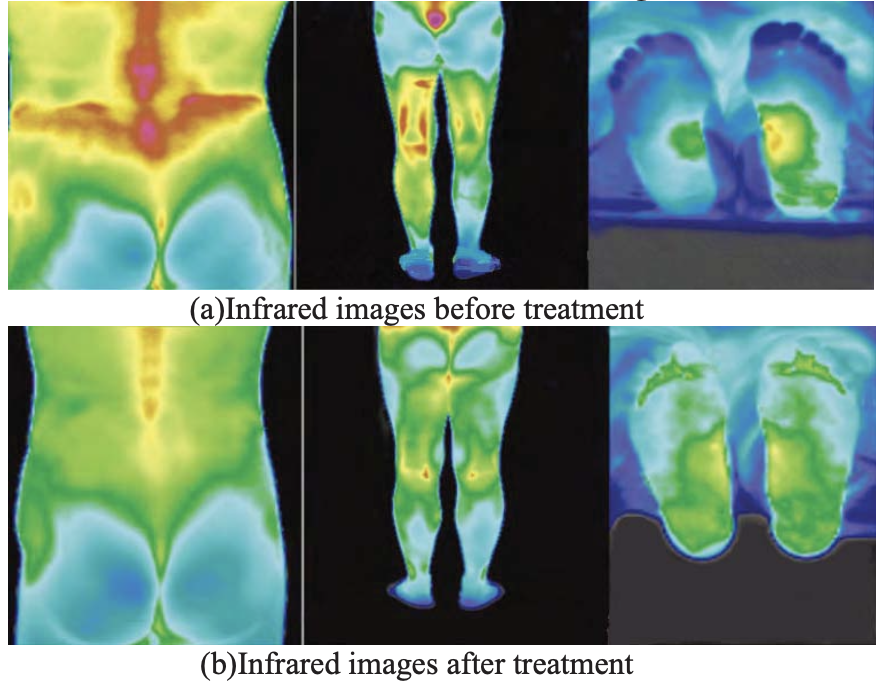
\includegraphics[width=0.7\textwidth]{Paper8.pic.jpg}
\caption{Comparison of infrared images of human body before and after treatment} 
\end{figure}
    
\noindent \textbf{Deep convolutional neural networks for thermal infrared object tracking}

\noindent This paper proposes an ensemble tracker for thermal infrared tracking (MCFTS) using multi-layer convolutional features based on correlation filters and convolutional neural networks, which can track targets in complete darkness(Qiao, 2017). The implementation of this document is mainly carried out through the introduction of the volume-based algorithm in thermal infrared images, the model update of the enhanced tracking algorithm and the experimental verification. Correlation filters are very popular in tracking methods because of their computationally efficient properties(Bolme, 2010), which is the core related work of this literature. It mainly includes 2D data and statistical graphs, mainly numerical data, and adds the expression of the dimension of robustness rank. In addition, it is evaluated by studying the algorithm documentation set, comparing with traditional convolutional neural network algorithms and verifying with experimental cases. Its representative image is as follows:

\begin{figure}[H]
\centering
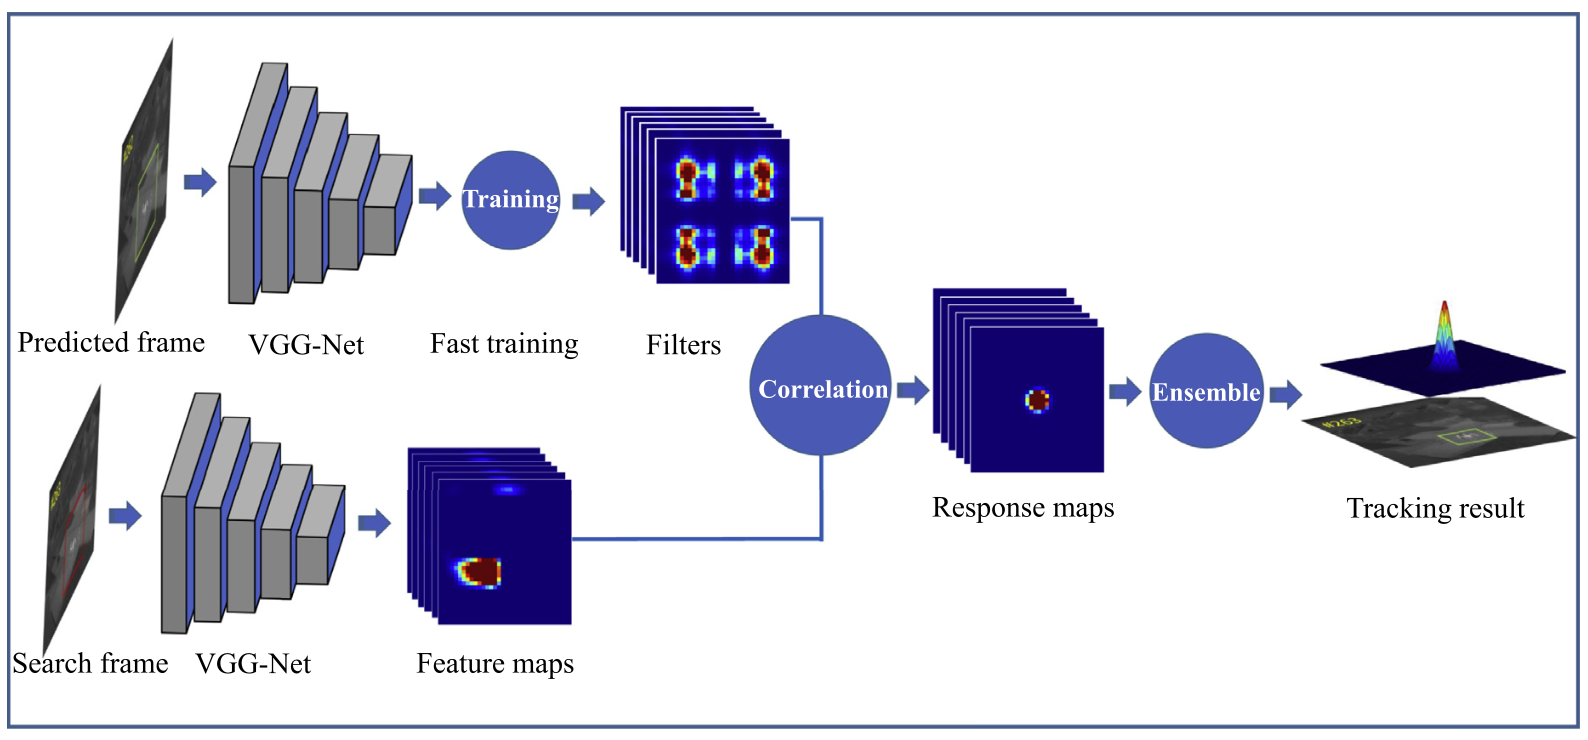
\includegraphics[width=0.7\textwidth]{Paper9.pic.jpg}
\caption{Method framework} 
\end{figure}

\noindent \textbf{Patient-Specific Pose Estimation in Clinical Environments}

\noindent This paper proposes a semi-automatic method for upper body pose estimation, which can improve the problem of calibration in noisy clinical environments(Chen, 2018). The Implementation of this document is mainly carried out through the steps of algorithm deployment and calculation formula introduction and experimental data visualization. The use of deep CNNs to automatically estimate joint positions during long-term recordings has been extensively studied(Pfister, 2015), which is the core related work of this literature. It contains 2D and 3D data, and adds time and space dimensions, and builds visual charts with numbers and vectors. Furthermore, it evaluates by studying algorithm files, simulations and comparative experiments. Its representative image is as follows:

\begin{figure}[H]
\centering
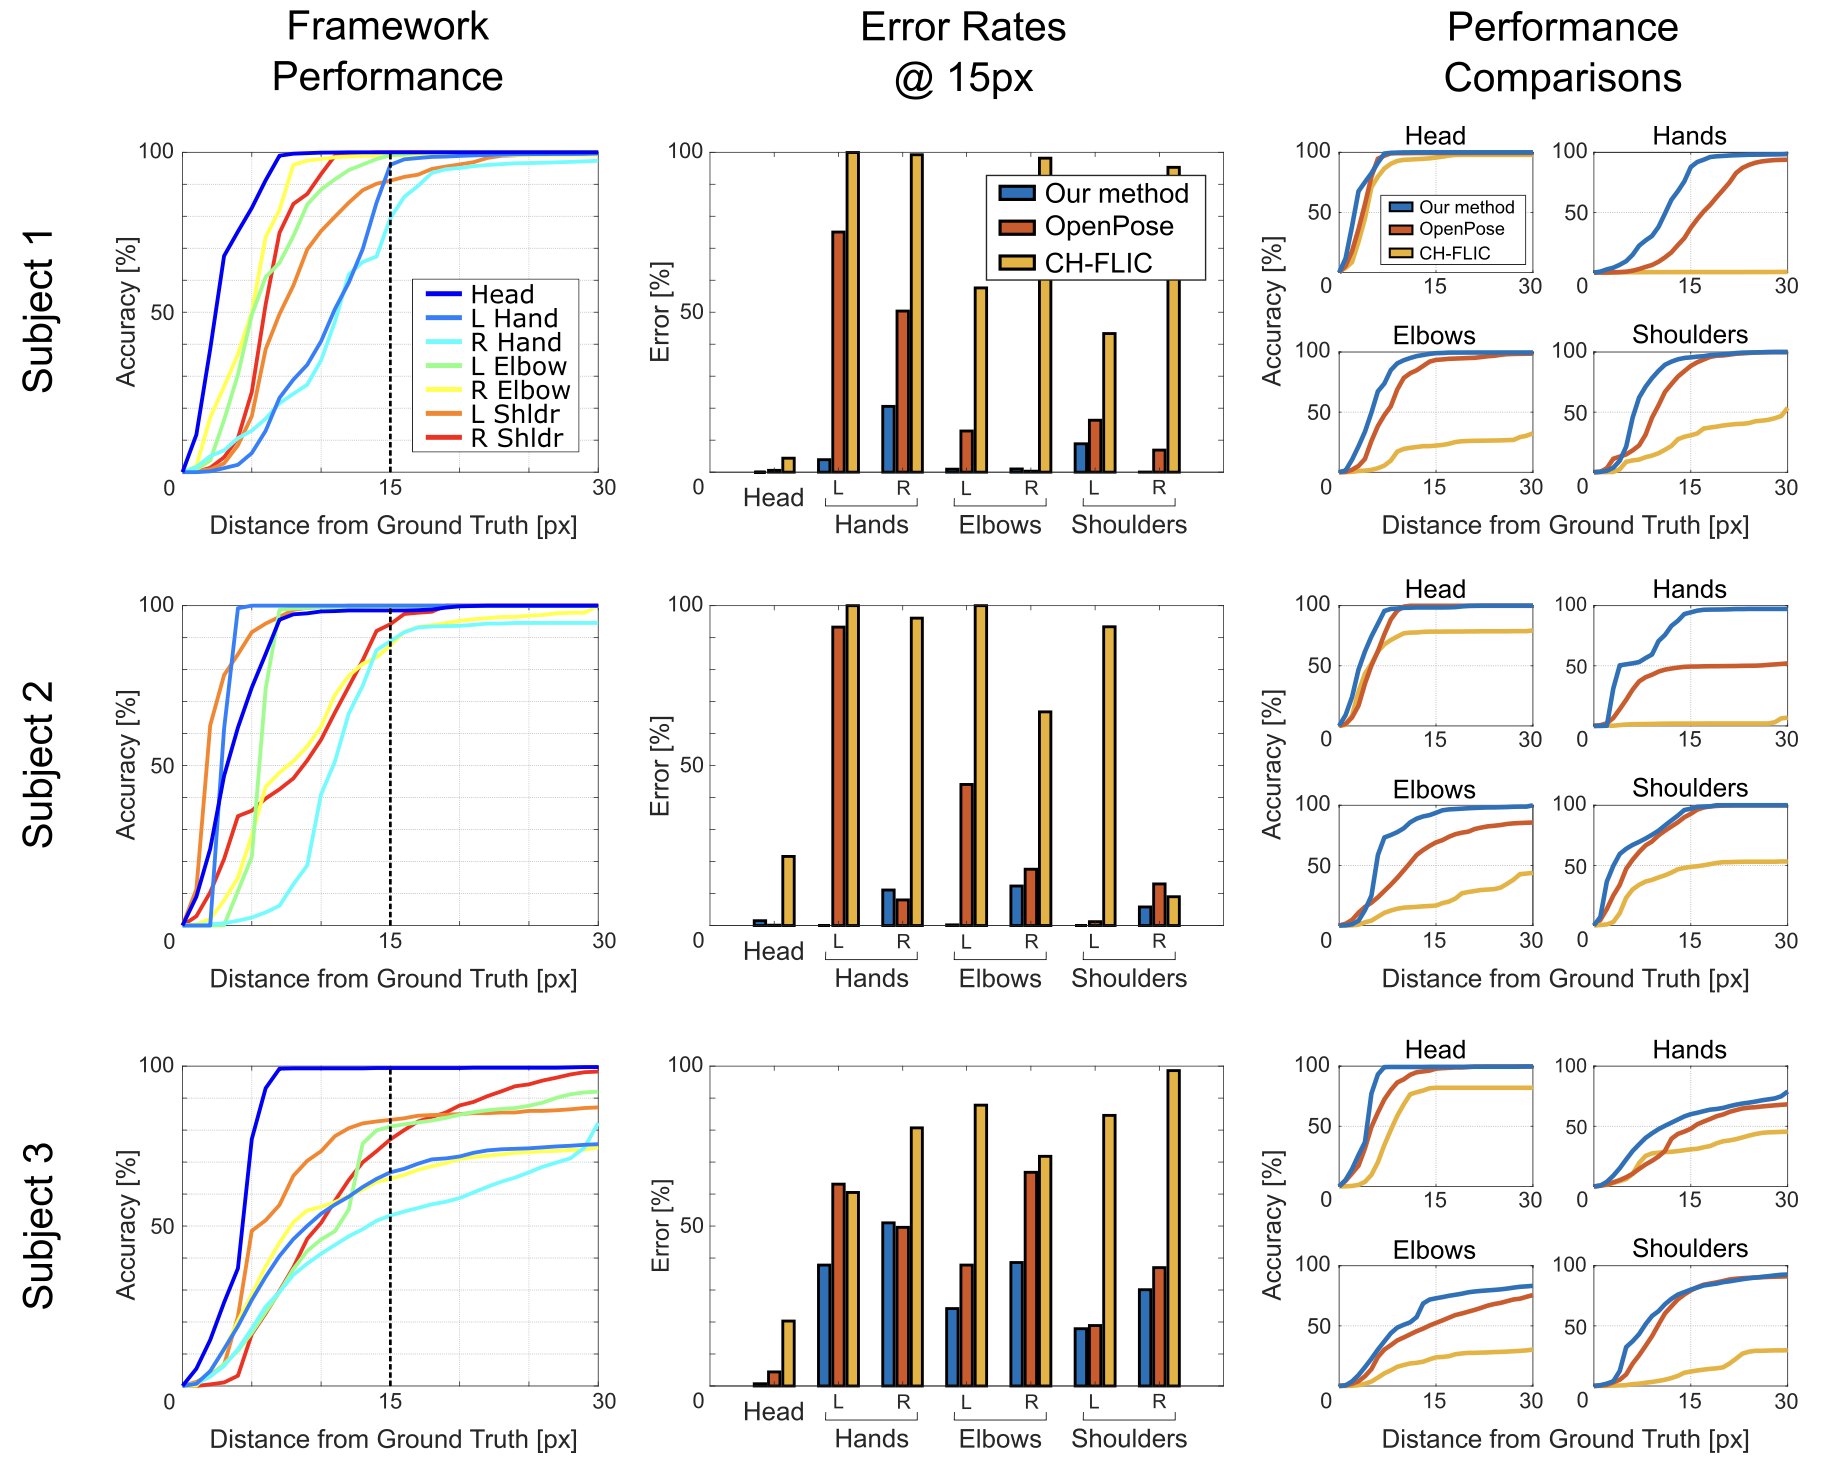
\includegraphics[width=0.7\textwidth]{Paper10.pic.jpg}
\caption{Comparison of pose estimation} 
\end{figure}

\newpage
\section{References}
Cheung, J.C.-W.; Tam, E.W.-C.; Mak, A.H.-Y.; Chan, T.T.-C.; Lai, W.P.-Y.; Zheng, Y.-P. Night-Time Monitoring System (eNightLog) for Elderly Wandering Behavior. Sensors 2021, 21, 704. https://doi.org/10.3390/s21030704

\noindent Wang X, Ellul J and Azzopardi G (2020) Elderly Fall Detection Systems: A Literature Survey. Front. Robot. AI 7:71. doi: 10.3389/frobt.2020.00071

\noindent D. Anderson, J. M. Keller, M. Skubic, X. Chen and Z. He, "Recognizing Falls from Silhouettes," 2006 International Conference of the IEEE Engineering in Medicine and Biology Society, New York, NY, USA, 2006, pp. 6388-6391, doi: 10.1109/IEMBS.2006.259594.

\noindent M. D. Solbach and J. K. Tsotsos, "Vision-Based Fallen Person Detection for the Elderly," 2017 IEEE International Conference on Computer Vision Workshops (ICCVW), Venice, Italy, 2017, pp. 1433-1442, doi: 10.1109/ICCVW.2017.170.

\noindent M. Brand and V. Kettnaker, "Discovery and segmentation of activities in video," in IEEE Transactions on Pattern Analysis and Machine Intelligence, vol. 22, no. 8, pp. 844-851, Aug. 2000, doi: 10.1109/34.868685.

\noindent Hua Zhong, Jianbo Shi and M. Visontai, "Detecting unusual activity in video," Proceedings of the 2004 IEEE Computer Society Conference on Computer Vision and Pattern Recognition, 2004. CVPR 2004., Washington, DC, USA, 2004, pp. II-II, doi: 10.1109/CVPR.2004.1315249.

\noindent M. F. A. Mushahar and N. Zaini, "Human Body Temperature Detection based on Thermal Imaging and Screening using YOLO Person Detection," 2021 11th IEEE International Conference on Control System, Computing and Engineering (ICCSCE), Penang, Malaysia, 2021, pp. 222-227, doi: 10.1109/ICCSCE52189.2021.9530864.

\noindent W. Yongqing, G. Zongqing, W. Shuonan and H. Ping, "The temperature measurement technology of infrared thermal imaging and its applications review," 2017 13th IEEE International Conference on Electronic Measurement \& Instruments (ICEMI), Yangzhou, China, 2017, pp. 401-406, doi: 10.1109/ICEMI.2017.8265833.

\noindent Qiao Liu, Xiaohuan Lu, Zhenyu He, Chunkai Zhang, Wen-Sheng Chen, Deep convolutional neural networks for thermal infrared object tracking, Knowledge-Based Systems, Volume 134, 2017, Pages 189-198, ISSN 0950-7051, https://doi.org/10.1016/j.knosys.2017.07.032.

\noindent K. Chen et al., "Patient-Specific Pose Estimation in Clinical Environments," in IEEE Journal of Translational Engineering in Health and Medicine, vol. 6, pp. 1-11, 2018, Art no. 2101111, doi: 10.1109/JTEHM.2018.2875464.

\noindent Bloom, D. E., Boersch-Supan, A., McGee, P., and Seike, A. (2011). Population aging: facts, challenges, and responses. Benefits Compens. Int. 41, 22.

\noindent H. Zhong, M. Visontai, J. Shi, “Detecting Unusual Activity in Video,”
IEEE Computer Society Conf. on Computer Vision and Pattern
Recognition, vol. 2, pp. 819-826, June 2004.

\noindent Ranasinghe, D.C.; Shinmoto Torres, R.L.; Hill, K.; Visvanathan, R. Low cost and batteryless sensor-enabled radio frequency identification tag based approaches to identify patient bed entry and exit posture transitions. Gait Posture 2014, 39, 118–123. [CrossRef]

\noindent N. Noury, A. Fleury, P. Rumeau, A. Bourke, G. O. Laighin, V. Rialle, and J. Lundy. Fall detection - Principles and Meth- ods. 2007 29th Annual International Conference of the IEEE Engineering in Medicine and Biology Society, pages 1663– 1666, 2007.

\noindent F. Jelinek, Statistical Methods for Speech Recognition. MIT Press, 1998.

\noindent C. Wren, A. Azarbayejani, T. Darrell, and A. Pentland. Pfinder: Real-time tracking of the human body. IEEE Transactions on Pattern Analysis and Machine Intelligence, 19(7):780–785, July 1997.

\noindent J. R. Hageman, “The Coronavirus Disease 2019 (COVID-19)”, Pediatr. Ann., vol. 49, no. 3, pp. e99–e100, 2020

\noindent Li Yunhong. Research on temperature measurement technology and application based on infrared thermal imager. Harbin: Harbin Institute of Technology, 2010.

\noindent D.S. Bolme, J.R. Beveridge, B.A. Draper, Y.M. Lui, Visual object tracking using adaptive correlation filters, in: IEEE Conference on Computer Vision and Pat- tern Recognition (CVPR), 2010, pp. 2544–2550.

\noindent T. Pfister, J. Charles, and A. Zisserman, ‘‘Flowing ConvNets for human pose estimation in videos,’’ in Proc. IEEE Int. Conf. Comput. Vis., Dec. 2015, pp. 1913–1921.

\end{document}


